In this supplementary material we highlight the use cases that \noah
is suited for, the in-situ chart representations within
the overview, \noah’s underlying system architecture,
and statistical significance results from our user study.
\section{\noah Use Cases}
As mentioned in Section~\ref{sec:design}, the goal of designing 
an overview interface is to 
not only enable seamless navigation 
but also to facilitate functionalities to help users visually seek information about the data. Therefore, we draw parallels to the typology of abstract visualization tasks~\cite{brehmer2013multi} to identify the use cases that \noah is best suited for. 
We are specifically interested in exploring the different task purposes mentioned in the typology. The task purposes can be specified at three different levels: consume and produce (high-level), search (mid-level), and query (low-level). Table~\ref{tab:scope} captures all three levels and highlights where \noah can be used.

\begin{table}[!htb]{\scriptsize}
\caption{Uses case of \noah.}
\label{tab:scope}
\centering
\begin{tabular}{c c}
\hline
Purpose & Use Cases   \\ \hline
\emph{Consume}         & \code{discover} (\checkmark), \code{present} (\checkmark), \code{enjoy} (\checkmark)\\
\emph{Produce}         & \code{create} (\checkmark), \code{annotate} ($\times$)\\
\emph{Search}            & \code{browse} (\checkmark), \code{explore (\checkmark)}, \code{locate} ($\times$), \code{lookup} ($\times$)\\
\emph{Query}    &  \code{identify} (\checkmark), \code{summarize} (\checkmark), \code{compare} (\checkmark)  \\ \hline
\end{tabular}
\end{table}

At a very high level, users may utilize \noah to verify some phenomenon in the data (\code{discover}) or consume the data for casual interest (\code{enjoy}). Example of \code{discover} includes a journalist trying to verify whether listings in Airbnb are run as hotels (see Section~\ref{sec:usage}). 
Moreover, users may utilize the overview to communicate details about the data (\code{present}). 
However, visualization tools are more suitable for such a purpose. 
Finally, users can customize (\code{create}) the overview to fit their exploration purpose. Here, the high-level goal is to \emph{Produce} a new representation. 
However, the present version of \noah does not allow users to add annotations, \eg visual cues, texts, to the overview (\code{annotate}).

Regardless of the high-level purposes, users may want to find elements of interest in the overview (\emph{search}) and seek additional details about those elements (\emph{query}). 
In Section~\ref{sec:ui}, we discussed the features and interactions supported by \noah and showed how these interactions enable users to \emph{search} and \emph{query} the data. Users can \code{browse} and \code{explore} the data using navigational operations, \eg clicking and zooming, to find elements of interest. 
Note that if users know either the identity or location of the information they are searching (\eg the name of the city in the Airbnb data), 
they can simply use traditional spreadsheet operations like \emph{VLOOKUP} (\code{lookup}) or \emph{CTRL+F} (\code{locate}) (see Table~\ref{tab:scope}). 
On the other hand, clicking or zooming is suitable when the identity or location of the information is unknown. Therefore, NOAH complements spreadsheets in accomplishing users’ \emph{search} goal via navigational operations. 
Once the user finds the elements of interest, they can further \code{summarize} the elements via aggregate columns, \code{compare} those elements, and \code{identify} the raw data corresponding to the summaries in the spreadsheet.




\section{Explaining the Chart Representations}

In this section, we explain the chart representation of all the
formula categories discussed in Section~\ref{sec:ui},
also displayed in Figure~\ref{fig:agg}.

\stitle{Summary.} The result of a \emph{summary} formula,
\eg \code{AVERAGE}, is depicted using a horizontal bar.
The bar represents
the range of the data subset the bin spans
with the minimum and maximum values
annotated within the chart. A vertical line is used to highlight
where the result lies within the range.
   
\stitle{Conditional.} The result of a \emph{conditional} formulae,
\eg \code{COUNTIF}, is depicted using a histogram.
The histogram captures the distribution of the attribute,
on which the formula has been applied,
\eg the \emph{availability} attribute discussed
in Section~\ref{sec:usage}.
Shading is used to de-emphasize data ranges
that do not satisfy the condition. A vertical line is used to highlight
where the result lies within the distribution.

\stitle{Frequency.} The result of a \emph{frequency} formula,
\eg \code{mode}, is also depicted using a histogram.
The bin in the histogram
that contains the result is rendered with ``orange'' color.
A vertical line is used to highlight
where the result lies within the distribution.

\stitle{Spread.} Finally, the result of a \emph{spread} formula,
\eg \code{mode}, is depicted using a histogram.
A similar shading technique as the \emph{conditional} formula is used to highlight the standard deviation. The mean of the is highlighted using a vertical line.

In the chart representation mode,
each entry of the aggregate column
contains one additional visual cue---a color bar
with shades of green on
the right of the chart (see Figure~\ref{fig:customize}).
The darker the color, the higher the value corresponding to that entry. 
Users can utilize the color intensity
to compare the results among different aggregate column entries.

\section{Implementation and  Architecture}
\label{sec:sys}
In this section, we provide an overview of the infrastructure of \noah. 
We integrate \noah as a data exploration plugin within{\scshape DataSpread}~\cite{dataspread}, 
an open-source scalable web-based spreadsheet.

\subsection{Underlying Data Structures}
As explained in Section~\ref{sec:ui}, the underlying data structure representing the overview is an in-memory equi-depth histogram. 
\noah constructs the histogram on demand based on the navigation attribute. 
In the beginning, only the highest granularity bins are constructed. 
As users perform ad-hoc interactions on the data, the interface is updated on the fly. 
For example, when a user zooms into a specific bin, 
\noah again constructs an equi-depth histogram 
on the data corresponding to that bin on demand.
To enable seamless integration of the overview 
with the spreadsheet data, we leverage the hierarchical positional indexes
used by {\scshape DataSpread}~\cite{datamodels} to access
the spreadsheet data. 
The index is essentially an
order statistics tree~\cite{datamodels} 
built on the position (\eg row number) of the spreadsheet data. 
For any given navigation attribute, a new positional index is constructed first. 
\noah then leverages the positional mapping to access the underlying data corresponding to the navigation attribute and constructs the histogram depicting the overview. 
Each bin in the histogram maintains positional information regarding its elements, \ie starting and ending index of each unique element in the bin (\eg cities in the Airbnb data).  
Therefore, \noah can be integrated into any 
spreadsheet and requires only access to the positional mapping structure of that spreadsheet.

\subsection{System Architecture}

\begin{figure}
    \centering
    %\vspace{-10pt}
    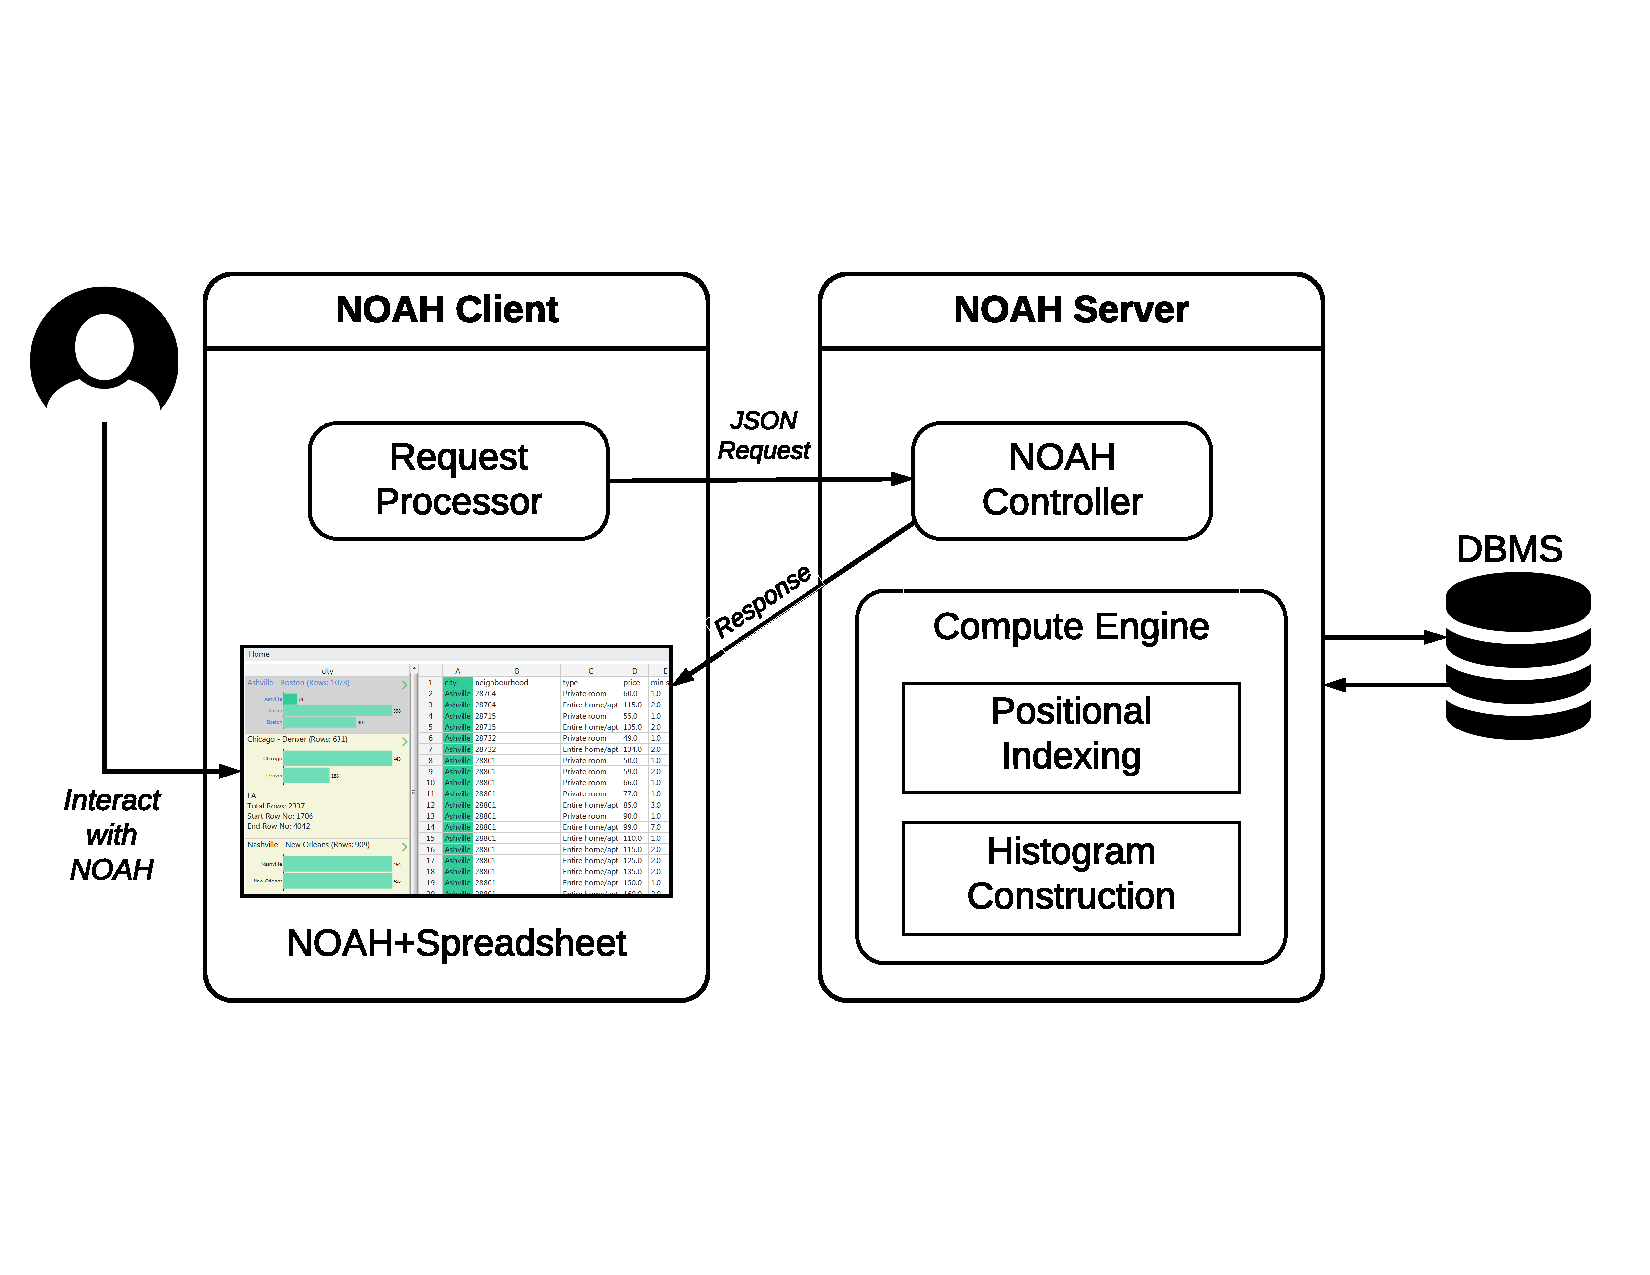
\includegraphics[trim=0 4cm 0 3cm,clip,width=\linewidth]{images/arch.pdf}
   \caption{System architecture.}
   \label{fig:arch}
 \end{figure} 

We now explain the system architecture of \noah. 
The \noah client is a web-based front-end that captures user input and renders both the navigation interface and the spreadsheet 
based on the results returned by the back-end. 
The front-end is responsible for capturing user input and rendering components of the navigation interface, \ie overview, aggregate column, and context bar. 
Given any interaction by the user on the front end, 
the \emph{request processor} issues a request to back end.
The back end navigation controller receives the request from the front end. 
After processing the request that corresponds to some front-end user interaction, 
the \emph{request processor} sends a response to the front-end encoded in \emph{json}. 
For requests involving the spreadsheet, \eg scrolling, 
the \emph{request processor} leverages the \emph{positional index} 
to access the spreadsheet data. 
For requests involving the navigation interface, \eg zoom in/out, 
the \emph{request processor} leverages the \emph{compute engine} to manage the equi-depth histogram on demand. 
The compute engine is also responsible for processing analytical operations. We leverage {\scshape DataSpread}’s built-in formula engine to support the analytical operations.


\section{Results}
In this section, we evaluate the statistical significance of the task performance results and survey responses presented in Section~\ref{sec:results}. 
\subsection{Statistical Significance: Task Performance}
Since we conducted our user study on a small population (20 participants), we further evaluated the statistical significance of the task performance results, \ie accuracy and completion time. 
To measure the significance of the task completion times, we ran \emph{Mann-Whitney's U test} (as completion times did not follow a normal distribution). \emph{For all of the tasks except the customize task, we found a significant effect of the tools, \ie the response times for the tasks significantly differed by the choice of the tool} (see Table~\ref{tab:statTest}). 
On the other hand, we ran the \emph{Fisher's exact test} that measures the statistical significance of categorical data (0/1 accuracy): \emph{only for steer tasks, the percentage of the accuracy of submissions significantly differed by the choice of the tool}. 

\begin{table}[!htb]{}
\vspace{-10pt}
\scriptsize
\caption{Statistical significance of submission time and accuracy comparisons between \noah and Excel. (*) indicates statistically significant.}
\label{tab:statTest}
\centering
\begin{tabular}{cccc}
\hline
Question & Category &  Time   &    Accuracy \\
& & ($p$ value) & ($p$ value) \\ \hline
$Q1$ & Steer & $\mathbf{0.0007}$ (*) &  $\mathbf{0.0033}$ (*)  \\
$Q2$ & Identify &   $\mathbf{2.49 \times 10^{-5}}$ (*) & $0.7475$ \\  
$Q3$ & Steer & $\mathbf{0.0043}$ (*) & $\mathbf{0.0202}$ (*) \\
$Q4$  & \cmpA & $\mathbf{0.0154}$ (*) & $1$ \\  
$Q5$ & \cmpB & $\mathbf{5.83 \times 10^{-6}}$ (*) & $0.48$\\
$Q6$ & Customize & $0.1207$ &    $0.0959$ \\\hline
\end{tabular}
\vspace{-10pt}
\end{table}

\subsection{Statistical Significance: Subjective Ratings}
We further conducted a statistical significance test---the \emph{Wilcoxon Signed-rank} test---on the survey responses which showed that for all the metrics, the ratings significantly differed by the choice of the tool, \ie \noah or Excel. The distribution of the ratings for none of the criteria followed a normal distribution.

\begin{table}[!htb]{\scriptsize}
\caption{Survey results. (*) indicates statistical significance. }
\label{tab:survey}
\centering
\begin{tabular}{|l|l|l|l|}
\hline
Metric &    \noah   &    Excel   & $p$ value \\ \hline
Ease of Learning &  $\mu = 5.75$, &    $\mu = 4.22$, & $\mathbf{1.49 \times 10^{-7}}$ (*) \\
& $\sigma = 1.02$ & $\sigma = 1.41$ & \\\hline
Speed of Use &    $\mu = 6.03$, & $\mu = 4.22$, & $\mathbf{1.68 \times 10^{-7}}$ (*)\\
& $\sigma = 0.99$ & $\sigma = 1.65$ & \\\hline  
Ease of Use    & $\mu = 5.88$, & $\mu = 4.33$, & $\mathbf{7.85 \times 10^{-6}}$ (*) \\
& $\sigma = 0.90$ & $\sigma = 1.71$ & \\\hline
Confidence    & $\mu = 5.50$, & $\mu = 4.60$, & $\mathbf{0.0096}$ (*)\\
& $\sigma = 1.79$ & $\sigma = 1.50$ & \\\hline  
Comprehensibility & $\mu = 5.60$, & $\mu = 4.48$, & $\mathbf{0.0006}$ (*)\\
& $\sigma = 1.27$ & $\sigma = 1.65$ & \\\hline
Satisfaction & $\mu = 5.48$, &    $\mu = 4.52$, & $\mathbf{0.0018}$ (*)\\
& $\sigma = 1.16$ & $\sigma = 1.49$ & \\\hline
\end{tabular}
\end{table}
